\documentclass[12pt, letterpaper]{article}
\usepackage{graphicx} % Required for inserting images
\usepackage{hyperref}
\usepackage{listings}
\usepackage{amssymb}
\usepackage{amsmath}
\usepackage[english]{babel}
\usepackage{nicefrac, xfrac}
\usepackage{mathtools}
\usepackage[table,xcdraw]{xcolor}
\definecolor{light-gray}{gray}{0.95}
\definecolor{sap}{RGB}{130, 36, 51}
\definecolor{lg}{RGB}{102, 161, 95}
\usepackage[paper=a4paper,left=20mm,right=20mm,bottom=25mm,top=25mm]{geometry}
\newcommand{\code}[1]{\colorbox{light-gray}{\texttt{#1}}}
\newcommand{\shelll}[1]{\colorbox{black}{\textcolor{white}{\texttt{#1}}}}
\newcommand{\shell}[1]{\colorbox{black}{\textcolor{white}{\texttt{casufrost@debian:$\sim$\$ #1}}}}
\newcommand{\codee}[1]{\colorbox{white}{\texttt{#1}}}
\newcommand{\acc}{\\\hphantom{}\\}
\newcommand{\comm}[1]{\color{lg}\textit{\hphantom{spaz}// \text{#1}}\color{black}}
\newcommand{\dete}{{\rightarrow}}
\newcommand{\fdot}{{\(\bullet\) }}
\newcommand{\boxedMath}[1]{\begin{tabular}{|c|}\hline \texttt{#1} \\ \hline\end{tabular} :}
\title{Progettazione di Algoritmi}
\author{Marco Casu}
\date{\vspace{-5ex}}
\begin{document}



\maketitle
\begin{figure}[h]
    \centering{
    
\includegraphics[width=1\textwidth ]{images/cop.jpg}
    }
\end{figure}
\newpage 
\tableofcontents
\newpage
\section{Grafi}
\subsection{Introduzione e Definizioni}
Un grafo, è una coppia $(V,E)$, dove $V$ è un insieme di \textit{nodi o vertici}, ed $E$ un 
insieme di archi che collegano i nodi. Un grafo è detto \textbf{semplice} se, per ogni 
coppia di nodi, essi sono collegati da al massimo un arco, e non esistono dei cicli su 
un singolo nodo. Nel corso ci occuperemo di \textit{visitare} i grafi in 
profondità ed in ampiezza (concetti che verranno ripresi più in avanti). \acc 
Un grafo, può vedere i suoi archi \textit{orientati}, in questo caso si dice che 
il grafo è \textbf{diretto}. Due nodi sono \textbf{adiacenti} se collegati da un arco, 
ed il \textbf{grado} di un nodo non è altro che il numero di nodi adiacenti ad esso.\begin{center}
    \includegraphics[width=1\textwidth ]{images/defGrafi.eps}
\end{center}
Esiste un problema classico dal 1700, noto come \textit{problema dei ponti di Königsberg}, 
si consideri la seguente città posta nei pressi di un fiume che la divide in diversi settori, collegati 
da appositi ponti, rappresentata con il seguente grafo :\begin{center}
    \includegraphics[width=1\textwidth ]{images/konigsberg.eps}
\end{center}
Ci si chiede se è possibile passeggiare per la città, visitando tutti i settori, senza passare per due volte 
sullo stesso ponte. Consideriamo il modello del grafo, una passeggiata su un grafo non è altro che una 
sequenza ordinata di vertici ed archi che si alternano, come : $v_0,e_1,v_1\dots, e_k,v_k$.
Esiste una passeggiata su questo grafo, ossia una sequenza che non vede ripetizioni degli archi?\acc 
\textbf{Osservazione} : Per visitare un nodo è necessario passare per due archi, uno entrante ed uno uscente. 
Se entriamo in un nodo di grado 3, resterà un arco non visitato, per visitarlo sarà necessario entravi nuovamente 
da tale arco, per poi uscire da un altro precedentemente già visitato (questo ovviamente se non si comincia la 
passeggiata dal nodo in questione).\acc 
Ci rende chiaro il seguente fatto : Se il grado di un nodo $x$ è dispari, a meno che la passeggiata non inizi 
o finisca su $x$, uno dei suoi archi verrà attraversato più di una volta. \textit{Eulero} studiò questo problema, 
si dice infatti che la passeggiata su un grafo è \textbf{euleriana} se non si passa 2 volte sulle stesso arco.\acc 
Si consideri però il seguente grafo :\begin{center}
    \includegraphics[width=1\textwidth ]{images/nonConnesso.eps}
\end{center}
Un grafo si dice \textbf{connesso} se, per ogni coppia di vertici, essi sono collegati da una passeggiata, 
ossia è possibile raggiungere un vertice partendo da un altro. Le precedenti osservazioni ci portano al 
seguente risultato.\acc 
\textbf{Teorema (Eulero)} : Un grafo ha una passeggiata euleriana se e solo se è connesso, ed 
esistono al massimo 2 vertici di grado dispari.\acc 
Il fatto che sono concessi 2 vertici di grado dispari, è dato dal fatto che essi saranno l'inizio e la fine 
della passeggiata.
\subsection{Rappresentazione Fisica}
Che struttura dati possiamo utilizzare per rappresentare un grafo? Vediamo due alternative : \begin{itemize}
    \item \textbf{Matrice di Adiacenza} - Utilizziamo una matrice $n\times n$, dove \(n\) è il numero di 
    nodi del grafo. Nella posizione \(i,j\) ci sarà 1 se il vertice \(v_i\) è adiacente al vertice 
    \(v_j\), altrimenti 0. Il costo di "\textit{check}" per l'adiacenza di due vertici è costante, basta 
    consultare un entrata della matrice, nonostante ciò, lo spazio che occupa tale rappresentazione è 
    \(O(n^2)\).
    \item \textbf{Liste di Adiacenza} - Ad ogni vertice del grafo è associata una lista, contenente tutti 
    i suoi vertici adiacenti, per controllare se due vertici sono adiacenti, è necessario fare una ricerca 
    lineare su tale lista, ed ha costo $\displaystyle O(\deg(v))$, dove \(v\) è il vertice sulla 
    quale si sta effettuando la ricerca, ed è ovviamente limitato da \(n-1\) (numero di vertici).\acc
    Le dimensioni della struttura dati sono $\displaystyle O\big(n + \sum_{v\in V(G)}\deg(v)\big)$.
\end{itemize}
Nel caso in cui un grafo dovesse vedere ogni vertice adiacente a tutti gli altri, la ricerca costerebbe 
\(O(n)\) e le dimensioni sarebbero \(O(n^2)\), ciò differisce però dal caso reale, la rappresentazione con 
liste di adiacenza risulta un buon compromesso fra costo computazionale e dimensioni.
Sarà usuale denotare \(m\) il numero di archi e \(n\) il numero di vertici.
Le liste di adiacenza occupano quindi spazio $O(n+m)$,  si osservi inoltre la 
seguente identià : $$\sum_{v\in V(G)}\deg(v)=2\cdot m\text{ dove }m:=|E|$$
\subsection{Ricerca di un Ciclo}
\textbf{Definizione} : Un \textit{ciclo} in un grafo, non p altro che un \textit{sottografo connesso} dove 
ogni vertice è di grado 2. Identifica un "cammino circolare", e la ricerca dei cicli nei grafi è un 
problema molto noto.\begin{center}
    \includegraphics[width=0.8\textwidth ]{images/ciclo.eps}
\end{center}
Consideriamo adesso un problema, vogliamo definire un algoritmo che, dato in input un grafo \(G=(V,E)\), dove ogni 
vertice ha grado maggiore o uguale a 2, restituisca in output un qualsiasi ciclo presente nel grafo, mantenendo 
un costo computazionele $O(n+m)=O(|V|+|E)$. 
\begin{quote}
    Si consideri la seguente \textit{idea} informale di soluzione : \end{quote}  
    Ogni vertice ha almeno 2 nodi adiacenti, è quindi sempre possibile entrare in un vertice ed uscirne da un
    arco diverso da quello dalla quale si è entrati. Si parte da un qualsiasi vertice nel grafo, e si procede 
    selezionando uno qualsiasi dei due nodi adiacenti successivi, almeno uno dei due non sarà quello dalla 
    quale si è entrati, procederemo in questa maniera camminando in maniera casuale sul grafo, finchè non troveremo 
    un nodo che è stato già visitato in precedenza, ciò indica che si è eseguito un cammino ciclico.\acc 
Utilizzeremo un vettore con lo scopo di salvare i nodi visitati, il ciclo sarà rappresentato 
dai nodi presenti nel vettore, partendo dall'ultimo elemento, continuando a ritroso fino a trovare il nodo 
identico all'ultimo. Si consideri il seguente esempio in cui gli archi sono contrassegnati dall'iterazione 
dell'algoritmo nella quale sono stati attraversati : 
\begin{center}
    \includegraphics[width=0.8\textwidth ]{images/algoCiclo.eps}
\end{center}
Una volta completato la ricerca del ciclo, elimineremo dal vettore tutti gli elementi a partire dal primo 
fino all'elemento antecedente a quello identico all'elemento finale. \begin{center}
    Pseudocodice 
\end{center}
\code{Input} : Un grafo $G=(V,E)$.\\
\code{Output} : I nodi di un sottografo di \(G\) che è un ciclo.\\\hphantom{}\\
\codee{CercaCiclo(graph G)\{}\\
\hphantom{ident}\codee{x = V[random]}\color{lg}\textit{// Un vertice a caso}\color{black}\\
\hphantom{ident}\codee{W=[x]}\color{lg}\textit{// Inizializzo il vettore output}\color{black}\\
\hphantom{ident}\codee{current = V}\\
\hphantom{ident}\codee{y=adiacente di x}\color{lg}\textit{// Un adiacente a caso}\color{black}\\
\hphantom{ident}\codee{next=y}\\
\hphantom{ident}\codee{while(next$\notin$ W)\{}\\
\hphantom{ident}\hphantom{ident}\codee{W.append(next)}\\
\hphantom{ident}\hphantom{ident}\codee{current=next}\\
\hphantom{ident}\hphantom{ident}\codee{if ($1^\circ$ adiacente di current$\ne$W[W.lenght-2])\{}
\color{lg}\textit{// Il penultimo}\color{black}\\
\hphantom{ident}\hphantom{ident}\hphantom{ident}\codee{next = $1^\circ$ adiacente di current}\\
\hphantom{ident}\hphantom{ident}\codee{\}else\{next = $2^\circ$ adiacente di current}\\
\hphantom{ident}\codee{\}}\\
\hphantom{ident}\codee{while(W[0]$\ne$next)\{}\\
\hphantom{ident}\hphantom{ident}\codee{W.remove(W[0])}\color{lg}\textit{// Rimuove il primo elemento}\color{black}\\
\hphantom{ident}\codee{\}}\\
\hphantom{ident}\codee{return W}\\
\codee{\}}\acc 
Qual'è la complessita di tale algoritmo? Entrambi i cicli \code{while} eseguono \(O(n)\) iterazioni, il 
fatto è che, nel primo ciclo while, il controllo \code{next$\notin$W} deve scorrere comunque tutto il vettore, 
rendendo il costo dell'algoritmo \(O(n^2)\), non rispettando le specifiche iniziali, ossia \(O(n+m)\).
\subsection{Cammini sui Grafi}
Un \textbf{cammino}, non è altro che una passeggiata su un grafo in cui non 
si passa mai più di una volta sullo stesso vertice, ossia una passeggiata 
senzza ripetizioni di vertici o archi. \acc 
\textbf{Osservazione} : Siano $x$ ed $y$ due nodi di un grafo, se esiste 
una passeggiata da $x$ ad $y$, allore esiste anche un cammino.\acc 
Nei grafi diretti vale la stessa regola, con ovviamente il vincola che bisogna rispettare 
l'orientazione degli archi. Un grafo diretto si dice \textbf{fortemente connesso} 
se, per ogni coppia di vertici \(x,y\), esiste un cammino da \(x\) ad \(y\)
e viceversa. \begin{center}
    \includegraphics[width=0.6\textwidth ]{images/fortConnesso.eps}
\end{center}
Un noto problema è il seguente, dato un grafo \(G\) e due veritici \(x,y\), esiste un cammino da \(x\) ad \(y\)? In generale, 
il carico di lavoro per controllare ciò, equivale al carico di lavoro necessario per controllare tutti i nodi che possono essere 
"raggiunti" partendo da \(x\).\acc 
Prendo quindi un vertici \(x\) e trovo tutti i vertici \(y\) per i quali esiste un cammino fra essi, per fare ciò, occorre 
\textbf{visitare} il grafo, e può essere fatto in due modi differenti.
\subsubsection{Depth-First Search}
Abbreviato \textbf{DFS}, tale algoritmo rappresenta la visita su un grafo in \textit{profondità}. Partendo da un qualsiasi 
vertice \(x\), inizio a visitare randomicamente uno dei vertici adiacenti, per poi proseguire da esso. Se ad un certo punto non 
vi sono nuovi vertici da visitare, si esegue il cosiddetto \textit{back tracking}, controllando i nodi a ritroso e cercando 
dei nuovi vertici. Risulta quindi naturale l'uso di uno \textit{stack} per poter implementare tale ricerca. L'algoritmo 
alla fine visiterà ogni nodo per la quale esiste un cammino dal nodo iniziale.
\begin{center}
    Pseudocodice
\end{center} 
\code{Input} : Un grafo $G=(V,E)$, ed un vertice \(x\).\\
\code{Output} : L'insieme dei vertici visitati partendo da \(x\).\\
\codee{DFS(graph G, vert x)\{}\\
\hphantom{ident}\codee{S : stack = \{x\}}\\
\hphantom{ident}\codee{Vis : set = [x]}\comm{l'insieme che conterrà l'output}\\
\hphantom{ident}\codee{while(S\(\ne\emptyset\))\{}\\
\hphantom{ident}\hphantom{ident}\codee{y=S.top()}\\
\hphantom{ident}\hphantom{ident}\codee{if(\(\exists\)z adiacente ad y\(\land \)x\(\notin\)Vis)\{}\\
\hphantom{ident}\hphantom{ident}\hphantom{ident}\codee{Vis.add(z)}\\
\hphantom{ident}\hphantom{ident}\hphantom{ident}\codee{S.push(z)}\\
\hphantom{ident}\hphantom{ident}\codee{\}}\\
\hphantom{ident}\hphantom{ident}\codee{else\{}\\
\hphantom{ident}\hphantom{ident}\hphantom{ident}\codee{S.pop()}\\
\hphantom{ident}\hphantom{ident}\codee{\}}\\
\hphantom{ident}\codee{\}}\\
\hphantom{ident}\codee{return Vis}\\
\codee{\}}\acc 
Esempio di applicazione (il nodo di partenza è il nodo 1) : \begin{center}
    \includegraphics[width=1\textwidth ]{images/DFS.eps}
\end{center}
L'output dell'algoritmo sarà proprio l'insieme \code{Vis}, contenente tutti i nodi raggiungibili dal vettore input, 
bisogna dimostrare che l'algoritmo sia corretto, mostrando che ogni vertice raggiungibile da \(x\) è in \code{Vis}.\acc 
\textbf{Dimostrazione} : Supponiamo per assurdo che vi sia un vertice \(y\) tale che, esiste un cammino da \(x\) ad 
\(y\) e che \(y\) non sia presente in Vis.
$$\exists y|x\rightarrow y\land y\notin\text{Vis}$$
Essendo \(x\) il vertice di partenza, esso sicuramente si troverà in Vis, per costruzione dell'algoritmo. Questo vuol dire che 
esiste un vertice nel cammino, per la quale vale la seguente proprietà : 
\begin{center}
    \includegraphics[width=0.7\textwidth ]{images/xxx.eps}
\end{center}
Essendo \(v_i\) in Vis, vuol dire che ad un certo punto è stato nel top 
dello stack, ma \(v_{i+1}\) è adiacente a \(v_i\), quindi da quest'ultimo l'algoritmo avrà selezionato 
ad un certo punto \(v_{i+1}\), per poi proseguire da esso, per costruzione, sarà inserito in Vis, ma ciò è 
in contraddizione con l'ipotesi iniziale che \(y\) non è in Vis. \(\blacksquare\)\acc 
Questo algoritmo presenta un problema cruciale, non è efficiente, infatti risulta particolarmente 
pesante il controllo \code{if(\(\exists\)z adiacente ad y\(\land \)x\(\ne\)Vis)}, che ha costo 
computazionale \(O(\deg(y))+O(n)\). L'algoritmo va migliorato, al posto di un set, è possibile utilizzare un 
array nella seguente maniera : sarà composto da \(n:=|V|\) elementi inizializzato con tutti 0, si avrà che
 \(array[i]=1\iff i\) fa parte dell'output.\begin{center}
    Pseudocodice
\end{center} 
\codee{DFS2(graph G, vert x)\{}\\
\hphantom{ident}\codee{S : stack = \{x\}}\\
\hphantom{ident}\codee{Vis : int[n] = [0,0\(\dots \)0]}\comm{L'array in questione}\\
\hphantom{ident}\codee{Vis[x]=1}\\
\hphantom{ident}\codee{while(S\(\ne\emptyset\))\{}\\
\hphantom{ident}\hphantom{ident}\codee{y=S.top()}\\
\hphantom{ident}\hphantom{ident}\codee{if(Vis[y.adiacenti[0]]==0)\{}\comm{Trova un adiacenta non ancora controllato}\\
\hphantom{ident}\hphantom{ident}\hphantom{ident}\codee{z=y.adiacenti[0]}\\
\hphantom{ident}\hphantom{ident}\hphantom{ident}\codee{Vis[z]=1}\\
\hphantom{ident}\hphantom{ident}\hphantom{ident}\codee{S.push(z)}\\
\hphantom{ident}\hphantom{ident}\hphantom{ident}\codee{y.adiacenti.remove(0)}\\
\hphantom{ident}\hphantom{ident}\codee{\}}\\
\hphantom{ident}\hphantom{ident}\codee{else\{}\\
\hphantom{ident}\hphantom{ident}\hphantom{ident}\codee{y.adiacenti.remove(0)}\\
\hphantom{ident}\hphantom{ident}\codee{\}}\\
\hphantom{ident}\hphantom{ident}\codee{if(y.adiacenti\(\ne\)0)\{S.pop()\}}\\
\hphantom{ident}\codee{\}}\\
\hphantom{ident}\codee{return Vis}\\
\codee{\}}\acc 
Si è nell'ipotesi in cui il grafo è implementato con le liste di adiacenza, infatti si noti come ogni vertice 
presenta il campo \code{adiacenti}. Per rendere più efficiente il tutto senza dover controllare ogni volta se un 
nodo è stato già visitato, semplicemente si rimuove dalla lista di adiacenza, ed ogni volta se ne prende il primo 
di tale lista che sicuramente non è stato ancora visitato, rendendo costante tale operazione.\acc 
Qual'è ora il costo computazionale? Quante  volte viene eseguito il ciclo \code{while}? Rispondere a ciò risulta 
difficile, piuttosto ci si chiede quanto lavoro devo fare nel ciclo per ogni vertice? Per ognuno di essi, si 
esegue un numero limitato di volte il comando \code{S.top()}. Nello specifico, si esegue tante volte quanto è il 
grado del vertice, risulta naturale che la complessità finale sia : 
$$O(n)+O\big( \sum_{v\in V(G)}\deg(v)\big)=O(n+|E|)=O(n+m)\text{ costo lineare}$$
Lo stesso algoritmo, si presta in maniera piuttosto naturale ad essere implementato in maniera ricorsiva, 
permettendo l'omissione dell'utilizzo di uno stack.\begin{center}
    Pseudocodice
\end{center} 
\codee{DFSRec(graph G, vert x,int[n] Vis)\{}\\
\hphantom{ident}\codee{Vis[x]=1}\\
\hphantom{ident}\codee{for each y\(\in\)x.adiacenti\{}\comm{per ogni adiacente di x}\\
\hphantom{ident}\hphantom{ident}\codee{if(Vis[y]==0)\{}\\
\hphantom{ident}\hphantom{ident}\hphantom{ident}\codee{DFSRec(G,y,Vis)}\\
\hphantom{ident}\hphantom{ident}\codee{\}}\\
\hphantom{ident}\codee{\}}\\
\codee{\}}\acc 
Il ciclo \code{for each y\(\in\)x.adiacenti} considera ogni adiacente di \(x\) una volta sola, facendo 
lo stesso lavoro di "cancellazione" dei vicini già controllati, la complessità rimane la medesima.\acc
Si considera la figura seguente, rappresentante una visita \textit{DFS} su un grafo :
\begin{center}
    \includegraphics[width=0.9\textwidth ]{images/AlberoDiVisita.eps}
\end{center}
Dal nodo di partenza, si inizia a visitare diversi nodi seguendo diversi percorsi, definiamo 
\textbf{albero di visita}, il sottografo generato, o composto dagli archi che utilizziamo per raggiungere i nuovi 
vertici non ancora visitati. In generale, un albero è un grafo connesso ed aciclico. Essendo che non si ritorna mai 
in un nodo già visitato due volte, nell'albero di visita non si creeranno cicli (rendendolo appunto un albero).\acc 
Possiamo applicare lo stesso algoritmo ai grafi diretti, l'unica considerazione da fare, è il controllo dell'ordine
di ogni arco. Consideriamo l'implementazione non ricorsiva.\begin{center}
    Pseudocodice
\end{center} 
\codee{DFSdiretto(graph G, vert x,)\{}\\
\hphantom{ident}\codee{S : stack = \{x\}}\\
\hphantom{ident}\codee{Vis : int[n] = [0,0\(\dots \)0]}\\
\hphantom{ident}\codee{Vis[x]=1}\\
\hphantom{ident}\codee{while(S\(\ne\emptyset\))\{}\\
\hphantom{ident}\hphantom{ident}\codee{y=S.top()}\\
\hphantom{ident}\hphantom{ident}\codee{if(\(\exists z|(y,z)\in E(G)\land \) Vis[z]==0)\{}\comm{l'arco ha la giusta orientazione}\\
\hphantom{ident}\hphantom{ident}\hphantom{ident}\codee{S.push(z)}\\
\hphantom{ident}\hphantom{ident}\hphantom{ident}\codee{Vis[z]=1}\\
\hphantom{ident}\hphantom{ident}\codee{\}}\\
\hphantom{ident}\hphantom{ident}\codee{else\{}\\
\hphantom{ident}\hphantom{ident}\hphantom{ident}\codee{S.pop()}\\
\hphantom{ident}\hphantom{ident}\codee{\}}\\
\hphantom{ident}\codee{\}}\\
\hphantom{ident}\codee{return Vis}\\
\codee{\}}\acc 
Anche questo algoritmo genera l'albero di visita, solo che avrà tutti gli archi, ordinati "verso il basso", ossia 
seguiranno l'orientazione che va dalla radice verso le foglie, tale albero è detto \textbf{arborescenza}.
\subsubsection{Componenti di un Grafo}
Se \(G\) è un grafo connesso, è ovvio che la DFS, qualsi voglia sia il vertice iniziale, restituirà sempre tutti 
i vertici del grafo. Se esso non dovesse essere connesso, restituirà un sottografo, precisamente il sottografo 
\textbf{componente} connesso che contiene il nodo input, i diversi sottografi componenti costituiscono una 
\textit{partizione} del grafo originale.\begin{center}
    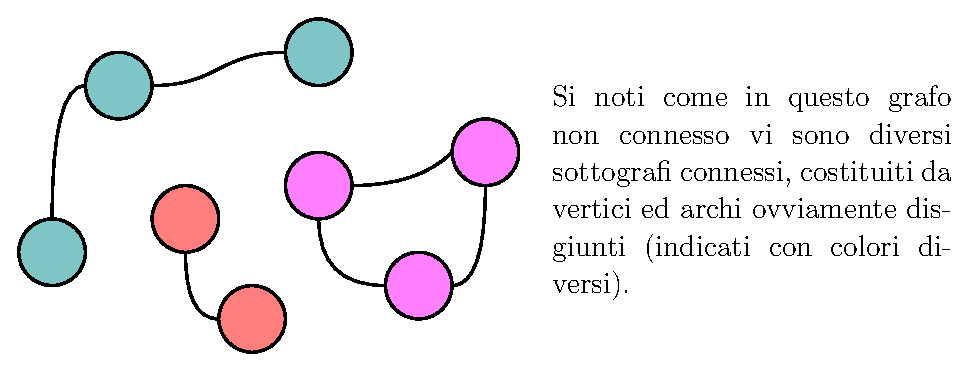
\includegraphics[width=0.9\textwidth ]{images/comp.eps}
\end{center}
Saper riconoscere le componenti di un grafo è un problema noto, che trova applicazione in svariati ambiti, ad esempio, 
nell'identificazione delle reti di amicizia in un social network, per capire se ci sono grandi gruppi di persone 
per i quali non vi è nemmeno 1 collegamento.\acc 
Il problema è il seguente, si vuole scrivere un algoritmo che identifichi tutte le componenti di un grafo, 
associando ad ogni vertice, un indice che ne indica la componente, dato un grafo \(G\), e due vertici 
\(x,y\), si vuole costruire 
un array Comp  tale che : \begin{center}
    Comp[\(x\)]=Comp[\(y\)]\(\iff\)\(x\) ed \(y\) sono nella stessa componente
\end{center}
Utilizziamo la versione ricorsiva del DFS, modificandola a dovere, sono necessarie 2 funzioni : \begin{center}
    Pseudocodice
\end{center} 
\codee{DFSRecComp(graph G, vert x,int[n] Comp, int index)\{}\comm{funzione di supporto}\\
\hphantom{ident}\codee{Comp[x]=index}\\
\hphantom{ident}\codee{for each y\(\in\)x.adiacenti\{}\comm{per ogni adiacente di x}\\
\hphantom{ident}\hphantom{ident}\codee{if(Comp[y]==0)\{}\\
\hphantom{ident}\hphantom{ident}\hphantom{ident}\codee{DFSRec(G,y,Comp,index)}\\
\hphantom{ident}\hphantom{ident}\codee{\}}\\
\hphantom{ident}\codee{\}}\\
\codee{\}}\acc 
\codee{Comp(graph G)\{}\comm{funzione principale da eseguire}\\
\hphantom{ident}\codee{Comp : int[n] = [0,0\(\dots \)0]}\\
\hphantom{ident}\codee{index = 0}\\
\hphantom{ident}\codee{for each x\(\in\)V(G)\{}\comm{per ogni vertice del grafo}\\
\hphantom{ident}\hphantom{ident}\codee{index++}\\
\hphantom{ident}\hphantom{ident}\codee{DFSRecComp(G,x,Comp,index)}\\
\hphantom{ident}\codee{\}}\\
\hphantom{ident}\codee{return Comp}\\
\codee{\}}
\subsubsection{Ordinamento Topologico}
Supponiamo che vi sia un progetto da completare, che viene diviso in \(n\) piccoli processi 
\(x_1,x_2\dots x_n\), e supponiamo che fra essi, vi siano delle dipendenze sull'ordine di completamento, ad 
esempio : \begin{itemize}
    \item Per essere completato \(x_1\), ha bisogno che siano completati \(x_2,x_3\)
    \item Per essere completato \(x_3\), ha bisogno che sia completato \(x_2\)
\end{itemize}
Dobbiamo pensare ad una programmazione dei processi che rispetti le dipendenze allo scopo di completare il progetto.
Nell'esempio dato, l'ordine corretto sarebbe \(x_2,x_3,x_1\). Utilizziamo un grafo diretto per modellizzare il 
problema : i processi saranno i vertici del grafo, e vi sarà un arco da \(x_i\) a \(x_j\) se \(x_i\) dipende 
da \(x_j\).\acc In questo modello, una programmazione dei processi non è altro che un ordine dei vertici 
del grafo, con la proprietà che tutti i vertici siano orientati "da destra verso sinistra".\begin{center}
    \includegraphics[width=0.3\textwidth ]{images/processiGrafo.eps}
\end{center}
\textbf{Osservazione} : Se in un grafo diretto vi è un ciclo, allora il grafo non ha tutti gli archi che vanno 
da destra verso sinistra. \acc 
\textbf{Dimostrazione} : Presumiamo che esista tale ordine, allora esiste un vertice \(x\) che è l'ultimo vertice 
di tale ordinamento, esiste quindi un arco \((y,x)\) per qualche \(y\), però, nonostante sia l'ultimo, 
data la presenza di un ciclo, deve esistere un arco uscente \((x,y)\), ma quindi l'ordine iniziale non è rispettato, 
causando una contraddizione. \(\blacksquare\)\acc 
Se in un grafo diretto vi è un ciclo, tutto il grafo non ammette la proprietà dell'orientazione degli archi. Tale 
proprietà è nota con il nome di \textbf{ordine topologico}, e l'assenza di un ciclo, è condizione necessaria 
e sufficiente per garantirla.\acc 
\textbf{Proposizione} : Se ogni singolo vertice di un grafo diretto ha almeno un arco uscente, allora 
esiste un ciclo.\acc 
\textbf{Dimostrazione} : Se esiste sempre un arco uscente, è sempre possibile, partendo da un vertice \(x\) spostarsi 
in un suo vertice adiacente, ciò significa che è possibile "camminare" all'infinito sul grafo, il fatto è che il 
numero di vertici è finito, quindi prima o poi si visiterà un vertice per una seconda volta, trovandosi in un 
ciclo.\begin{center}
\includegraphics[width=0.7\textwidth ]{images/controEsempio.eps}
\end{center}
\textbf{Corollario} : Se non esiste alcun ciclo in un grafo, allora esiste almeno un vertice che non ha 
archi uscenti.\acc 
Per ottenere un cosiddetto \textbf{ordinamento topologico}, posso considerare il seguente algoritmo : Si ha un 
grafo diretto \(G\), sprovvisto di cicli, si sceglie un qualsiasi vertice privo di archi uscenti, si inserisce 
in una lista per poi eliminarlo dal grafo (insieme a tutti i suoi archi associati), dopo ciò, si 
ri-esegue l'operazione, inserendo ogni volta il vertice nella prima posizione della lista.\acc Tale algoritmo risulta 
parecchio utile, si pensi all'ordinamento topologico applicato al grafo di serializzazione nell'ambito 
del controllo della concorrenza 
(trattato nel corso di \href{https://github.com/CasuFrost/University_notes/blob/main/Secondo%20Anno/Primo%20Semestre/Basi%20di%20Dati%201/Latex%20source%20file/Basi%20di%20Dati%20modulo%201.pdf}{Basi di Dati 1}).
\begin{center}
    Pseudocodice
\end{center}
\codee{OrdinamentoTopologico(graph G)\{}\comm{il grafo è diretto}\\
\hphantom{ident}\codee{L : list}\comm{una lista vuota, sarà l'output dell'algoritmo}\\
\hphantom{ident}\codee{while(G\(\ne\emptyset\))\{}\\
\hphantom{ident}\hphantom{ident}\codee{x=v\(\in\)V(G)|v.adiacentiOut=\(\emptyset\)}\comm{un vertice senza archi uscenti}\\
\hphantom{ident}\hphantom{ident}\codee{L.insert(x)}\\
\hphantom{ident}\hphantom{ident}\codee{G.delete(x)}\\
\hphantom{ident}\codee{\}}\\
\hphantom{ident}\codee{return L}\\
\codee{\}}\begin{center}
    \includegraphics[width=1\textwidth ]{images/ordTopologico.eps}
    \end{center}
Il \textit{problema} di questo algoritmo è il suo costo computazionale, di fatto è troppo dispendioso : Per 
controllare se un vertice non ha archi uscenti, si è in \(O(n)\), inoltre il ciclo \code{while} controlla 
tutti i vertici, quindi si è nuovamente in \(O(n)\).    \acc  La cancellazione di un vertice risulta dispendiosa, in 
quanto bisona eliminare anche tutti gli archi associati, ossia, eliminare il vertice da tutte le liste 
di adiacenza degli altri vertici, il numero di controlli dipende dal grado di ogni vertice,
quindi costa \(O(m)\). In totale, l'intero algoritmo ha una complessità \(O(n\cdot(n+m))\), vorremmo riuscire 
ad ottenere lo stesso output in tempo lineare.
\subsubsection{Contatore nel DFS e Relazioni sull'Arborescenza}
Vogliamo considerare un estensione del normale DFS, consideriamo un contatore, denotato \code{cc}, tale contatore, 
verrà incrementato ogni qual volta verrà visitato per la prima volta un nuovo nodo.\acc Consideriamo inoltre, due nuove 
funzioni \(t:V(G)\rightarrow\mathbb{N}\) e \(T:V(G)\rightarrow\mathbb{N}\), sia \(v\) un vertice, \(t(v)\) sarà uguale al valore 
del contatore \code{cc} nel momento in cui \(v\) viene visitato per la prima volta, invece \(T(v)\) sarà uguale al valore 
del contatore \code{cc} nel momento in cui \(v\) viene visitato per l'ultima volta, ossia quando esso viene rimosso dallo stack.\acc 
\textbf{Osservazione} : \begin{itemize}
    \item Per ogni coppia di vertici \(v,u\), si ha che \(t(v)\ne t(u)\)
    \item Per ogni vertice \(v\), si ha che \(t(v)\le T(V)\)
    \item Sia \(v\) un vertice, se \(t(v)=T(V)\), allora \(v\), è una foglia nell'albero di visita derivante dall'applicazione 
    del DFS.
    \item Sia \(n\) il numero di vertici e \(v_0\) la radice dell'albero di visita, si ha che \(t(v_0)=1\land T(v_0)=n\).
\end{itemize}
Esempio di applicazione dell'algoritmo (si parte dal vertice \(1\)) : \begin{center}
    \includegraphics[width=1.05\textwidth ]{images/dfsContatore.eps}
    \end{center}
Ad ogni vertice \(v\), è associato un \textit{intervallo} \([t(v),T(v)]\), gli intervalli di vertici diversi possono 
essere confrontati, e si ricade sempre in uno dei seguenti casi.\acc 
\textbf{Osservazione} : Siano \(v\) e \(u\) due vertici distinti del grafo, uno dei seguenti punti è sempre vero:\begin{itemize}
    \item \(i)\) $[t(v),T(v)]\subseteq[t(u),T(u)]$
    \item \(ii)\) $[t(v),T(v)]\supseteq[t(u),T(u)]$
    \item \(iii)\) $[t(v),T(v)]\cap[t(u),T(u)]=\emptyset$
\end{itemize}
\textbf{Dimostrazione} : Il quarto ed ultimo caso possibile, sarebbe un intersezione del tipo: $$
t(u)<t(v)\le T(u)<t(v)$$ Basta dimostrare che questa casistica non può verificarsi. Se \(u\) è stato inserito 
nello stack prima di \(v\), si avrà che \(T(u)\ge t(v)\), questo implica che \(u\) era già nello stack quando 
\(v\) è stato inserito, ma allora è impossibile togliere \(u\) prima di \(v\), e necessariamente \(T(u)>T(v)\). \(\blacksquare\)\acc 
Adesso, consideriamo il grafo sulla quale è stato applicato il nuovo DFS con contatore, e consideriamo gli archi che \textit{non appartengono} 
all'arborescenza, ossia gli archi che non sono stati attraversati durante il DFS (nell'immagine esplicativa precedente, quelli colorati in 
azzurro). \acc 
Vi è un fatto interessante, consideriamo tutti un qualsiasi arco non facente parte dell'arborescenza, esso indica due vertici \((v,u)\), 
e tali vertici posseggono gli intervalli che possono essere messi in relazione, ricadendo in uno dei 3 casi prima citati.\acc Gli archi 
non facenti parte dell'arborescenza, se considerati nell'arborescenza, potranno essere di 3 tipi, o partire da un vertice ed andare 
verso un suo antenato, o partire da un vertice ed andare 
verso un suo successore, oppure attraversare due vertici di due diramazioni differenti, in effetti, riguardo la relazione 
di intervalli prima citata, si ha che : \begin{itemize}
    \item Se i due vertici dell'arco ricadono nel punto \((i)\), allora l'arco va da un antenato ad un discendente (\textbf{arco in avanti}).
    \item Se i due vertici dell'arco ricadono nel punto \((ii)\), allora l'arco va da un discendente ad un antenato  (\textbf{arco all'indietro}).
    \item Se i due vertici dell'arco ricadono nel punto \((iii)\), allora l'arco attraversa due diramazioni differenti  (\textbf{arco di attraversamento}).
\end{itemize}
Riguardo il grafo del precedente esempio : \begin{center}
    \includegraphics[width=1.05\textwidth ]{images/archiArborescenza.eps}
    \end{center}
Si noti come l'arco che va dal vertice 8 al vertice 9, è un \textit{arco all'indietro}, infatti gli intervalli dei due 
vertici ricadono nel secondo caso : \([9,9]\supseteq[7,9]\).\acc  
Si noti come l'arco che va dal vertice 2 al vertice 4, è un \textit{arco in avanti}, infatti gli intervalli dei due 
vertici ricadono nel primo caso : \([2,6]\subseteq[6,6]\).\acc  
Si noti come l'arco che va dal vertice 7 al vertice 5, è un \textit{arco di attraversamento}, infatti gli intervalli dei due 
vertici ricadono nel terzo caso : \([8,9]\cap[4,5]=\emptyset\).\acc  
Se dovessi applicare lo stesso algoritmo ai grafi non diretti, non si potrebbe definire una relazione di antenato-discendente, 
in quanto ogni arco è percorribile per entrambe le direzioni, quindi i casi \((i)\) e \((ii)\) indicherebbero la stessa 
situazione.\acc 
Inoltre, è impossibile che, per due nodi \(u,v\) si verifichi che $[t(v),T(v)]\cap[t(u),T(u)]=\emptyset$, quindi  
il caso \((iii)\) è impossibile.\acc 
\textit{\textbf{Esercizio}} : Si vuole dare lo pseudocodice di una modifica del DFS, che restituisca in output 3 liste, una contenente 
gli archi in avanti, una quelli all'indietro, ed una gli archi di attraversamento.\begin{center}
    Pseudocodice
\end{center}
\codee{DFSconArchi(graph G, vert x,)\{}\comm{il grafo è diretto}\\
\hphantom{ident}\codee{int cc=1}\\
\hphantom{ident}\codee{t : int[n]} \comm{array lungo \(n\) inizializzato a zero}\\
\hphantom{ident}\codee{T : int[n]}\comm{array lungo \(n\) inizializzato a zero}\\
\hphantom{ident}\codee{t[x]=1}\\
\hphantom{ident}\codee{T[x]=|V(G)|}\\
\hphantom{ident}\codee{S : stack = \{x\}}\\
\hphantom{ident}\codee{Vis : int[n] = [0,0\(\dots \)0]}\\
\hphantom{ident}\codee{Vis[x]=1}\\
\hphantom{ident}\codee{while(S\(\ne\emptyset\))\{}\\
\hphantom{ident}\hphantom{ident}\codee{y=S.top()}\\
\hphantom{ident}\hphantom{ident}\codee{if(\(\exists z|(y,z)\in E(G)\land \) Vis[z]==0)\{}\comm{l'arco ha la giusta orientazione}\\
\hphantom{ident}\hphantom{ident}\hphantom{ident}\codee{S.push(z)}\\
\hphantom{ident}\hphantom{ident}\hphantom{ident}\codee{c++}\\
\hphantom{ident}\hphantom{ident}\hphantom{ident}\codee{t[z]=cc}\\
\hphantom{ident}\hphantom{ident}\hphantom{ident}\codee{Vis[z]=1}\\
\hphantom{ident}\hphantom{ident}\codee{\}}\\
\hphantom{ident}\hphantom{ident}\codee{else\{}\\
\hphantom{ident}\hphantom{ident}\hphantom{ident}\codee{S.pop()}\\
\hphantom{ident}\hphantom{ident}\hphantom{ident}\codee{T[z]=cc}\\
\hphantom{ident}\hphantom{ident}\codee{\}}\\
\hphantom{ident}\codee{\}}\\
\hphantom{ident}\codee{A : graph = arborescenza generata dal DFS}\\
\hphantom{ident}\codee{A' : graph = G-A}\comm{il complementare dell'arborescenza}\\
\hphantom{ident}\codee{av : list}\\
\hphantom{ident}\codee{ind : list}\\
\hphantom{ident}\codee{att : list}\\
\hphantom{ident}\codee{for each (x,y)\(\in\)E(A')\{}\\
\hphantom{ident}\hphantom{ident}\codee{switch(t[x],T[x],t[y],T[y])\{}\\
\hphantom{ident}\hphantom{ident}\hphantom{ident}\codee{$[t(v),T(v)]\subseteq[t(u),T(u)]$ : sv.append((x,y))}\comm{si ricade nel primo caso}\\
\hphantom{ident}\hphantom{ident}\hphantom{ident}\codee{$[t(v),T(v)]\supseteq[t(u),T(u)]$ : ind.append((x,y))}\comm{si ricade nel secondo caso}\\
\hphantom{ident}\hphantom{ident}\hphantom{ident}\codee{$[t(v),T(v)]\cap[t(u),T(u)]=\emptyset$ : att.append((x,y))}\comm{si ricade nel terzo caso}\\
\hphantom{ident}\hphantom{ident}\codee{\}}\\
\hphantom{ident}\codee{\}}\\
\hphantom{ident}\codee{return av,ind,att}\\
\codee{\}}\acc 
\end{document}
